\documentclass[12pt]{article}
\usepackage{tikz}

\begin{document}

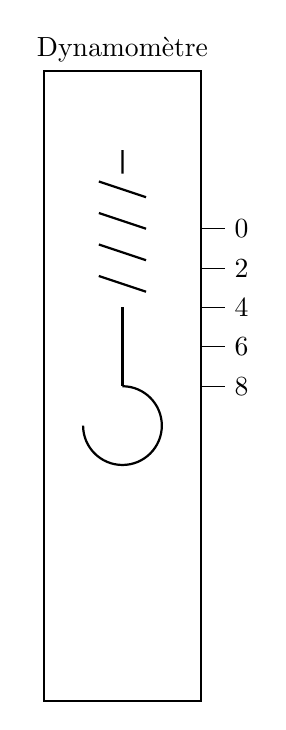
\begin{tikzpicture}[scale=1]

% Corps du dynamomètre
\draw[thick] (0,0) rectangle (2,8);

% Ressort
\draw[thick]
(1,7) -- (1,6.7)
(0.7,6.6) -- (1.3,6.4)
(0.7,6.2) -- (1.3,6.0)
(0.7,5.8) -- (1.3,5.6)
(0.7,5.4) -- (1.3,5.2)
(1,5.0);

% Crochet
\draw[thick] (1,5) -- (1,4);
\draw[thick] (1,4) arc (90:-180:0.5);

% Graduation
\foreach \y/\n in {6/0,5.5/2,5/4,4.5/6,4/8} {
  \draw (2,\y) -- (2.3,\y);
  \node[right] at (2.3,\y) {\n};
}

\node[above] at (1,8) {Dynamomètre};

\end{tikzpicture}

\end{document}